% appendix_experiments.tex: the rule-based experiments: posterior summaries under a flat prior (moved from Section 3.4), the payment path of every treatment and the p-value curve of every pair.
\section{The Rule-Based Experiments: Posterior Summaries and Exhibits}\label{appendix:experiments}

This appendix reports, for the rule-based experiments of Section \ref{sec:quasi}, the posterior summaries of the rate under a flat prior, the payment path of every treatment arm, and the $p$-value curve of every pair together with the near-horizon responses across settings and Indarte's pair as the model produces it.

\subsection{The treatments and the model's estimate from each pair}

\begin{table}[H]
\centering
\caption{Rule-based experiments as payment-path treatments, and the model's estimate from each pair}
\label{tab:experiments}
\resizebox{\textwidth}{!}{\begin{tabular}{lllllll}
\toprule
\multicolumn{7}{l}{\textit{Panel A: treatments as payment-path changes}} \\
Study & Treatment & Type & Far payments at & Outcome & Effect, pp (s.e.) & Base, \% \\
\midrule
\citet{ganong_liquidity_2020} & Principal forgiveness, payments fixed 5 years & relief & 5--26 years & 90+ days delinquent at any point, modi & +1.20 (3.18) & 19.0 \\
\citet{ganong_liquidity_2020} & Deeper payment reduction, maturity to 40 years & rescheduling & 22--40 years & 90+ days delinquent within two years o & -0.38 (0.08) & 32.1 \\
\citet{indarte_moral_2023} & Seizable home equity at filing & value of default & at decision & Chapter 7/13 filing in the quarter & -0.019 (0.0024) & 0.7 \\
\citet{indarte_moral_2023} & ARM reset: lower payment for 12 months & relief & within 1 year & filing in each of the 12 months after  & -0.21 (0.06) & 0.7 \\
\citet{dobbie_targeted_2020} & Interest write-down: last 10 payments forgiven & relief & 3.5--4.3 years & bankruptcy filing within 5 years & -3.00 (0.90) & 10.5 \\
\citet{dobbie_targeted_2020} & Payment cut, 18 extra months, fees up & rescheduling & 4.3--5.8 years & bankruptcy filing within 5 years & +2.30 (1.10) & 10.5 \\
\citet{dobbie_targeted_2020} (median) & Write-down: last 4 payments forgiven & relief & 3.8--4.2 years & bankruptcy filing within 5 years & -0.99 (0.52) & 10.4 \\
\citet{dobbie_targeted_2020} (median) & Payment cut, 4 extra months & rescheduling & 4.2--4.5 years & bankruptcy filing within 5 years & +0.70 (0.42) & 10.4 \\
\citet{fiorin_moratorium_2026} & 3-month deferral, fee, 3 payments after maturity & rescheduling & 6--8 months & loan repaid in full & +0.30 (1.30) & 42.0 \\
\citet{fuster_payment_2017} & 5/1 IO ARM reset: rate $-$3 pp, payment halved & relief (single arm) & from reset on & first 60-day delinquency & -56.30\% (3.00) & 1.7 \\
\citet{keys_mortgage_2014} & Agency 5/1 vs 7/1 reset: $-$\$125, $-$\$164 per month & relief (single arm) & years 1--2 & 60+ day mortgage delinquency, two year & -1.80 (1.00) & 4.5 \\
\citet{agarwal_policy_2017} & HAMP modification: $-$25\% payment, 5 years & relief, then step-up & years 1--5 & foreclosure completed within one year  & -12.45 (0.39) & -- \\
\midrule
\multicolumn{7}{l}{\textit{Panel B: the test of each pair against the model (joint test on the two arms; grid of $\rho$ from 0 to 3 by 0.01; decisions aggregated over the outcome window; survival from the study's exit hazards)}} \\
Pair & $\rho$ best fit & $p$ at $\rho = 0.02$ & $p$ at the estimate & $p$ at 0.22 & $\rho$ consistent at 5\% & $\rho$ consistent at 1\% \\
\midrule
Dobbie--Song pair (max arms), $\lambda_s$ profile & 0.00 & 0.925 & 0.734 & 0.538 & [0.00, 1.20] & [0.00, 2.84] \\
\quad same, arms correlated 0.5 & 0.00 & 0.938 & 0.774 & 0.597 & [0.00, 1.24] & [0.00, 2.24] \\
\quad same, constant $\lambda = 0.2$ & 0.05 & 0.913 & 0.865 & 0.622 & [0.00, 0.99] & [0.00, 1.97] \\
Dobbie--Song pair (median arms), $\lambda_s$ profile & 0.00 & 0.628 & 0.575 & 0.517 & [0.00, 3.00] & [0.00, 3.00] \\
Ganong--Noel pair, $\lambda_s$ profile & 3.00 & 0.246 & 0.396 & 0.502 & [0.00, 3.00] & [0.00, 3.00] \\
\bottomrule
\end{tabular}}
\vspace{0.5em}
\begin{minipage}{0.95\textwidth}
\small \textit{Notes:} Panel A codes each treatment as the change in dollars owed by month relative to the study's control; effects are the studies' reported estimates on the outcome and horizon shown. Panel B tests each pair of arms from the same population on the grid of $\rho$ from 0 to 3 by 0.01: the joint $\chi^2(1)$ distance of the two reported effects from the model's line effect$_1 = r(\rho)\,$effect$_2$, with $r(\rho)$ the ratio of the arms' weighted payment changes under exponential discounting, aggregated over the decision months of each study's outcome window with the study's own event timing (equation \eqref{eq:window}), survival from the study's own exit hazards (the re-default or filing hazard scaled by the uncured share, plus the payoff hazard), and the marginal-utility profile of equation \eqref{eq:lambda_p} at the study population's baseline rate and payment share, through Indarte's $0.2$; the rows marked ``same'' repeat the test with the two arms' sampling errors correlated at 0.5 (their covariance is not reported and the main rows treat them as independent) and with a constant $\lambda = 0.2$. The reference rates are the 2 percent social discount rate, the paper's estimate, and the laboratory median of 0.22. Sets are the rates on the grid not rejected at the stated level, as unions of intervals where they are not connected. Indarte's pair identifies $\lambda$ and is not tested for $\rho$.
\end{minipage}
% replication: Code/local/experiments_ledger.R, Code/exhibits/make_experiments_table.py; external/experiments_paths.csv, external/experiments_estimates.csv, results/experiments_rho_summary.csv
\end{table}

\begin{figure}[H]
\centering
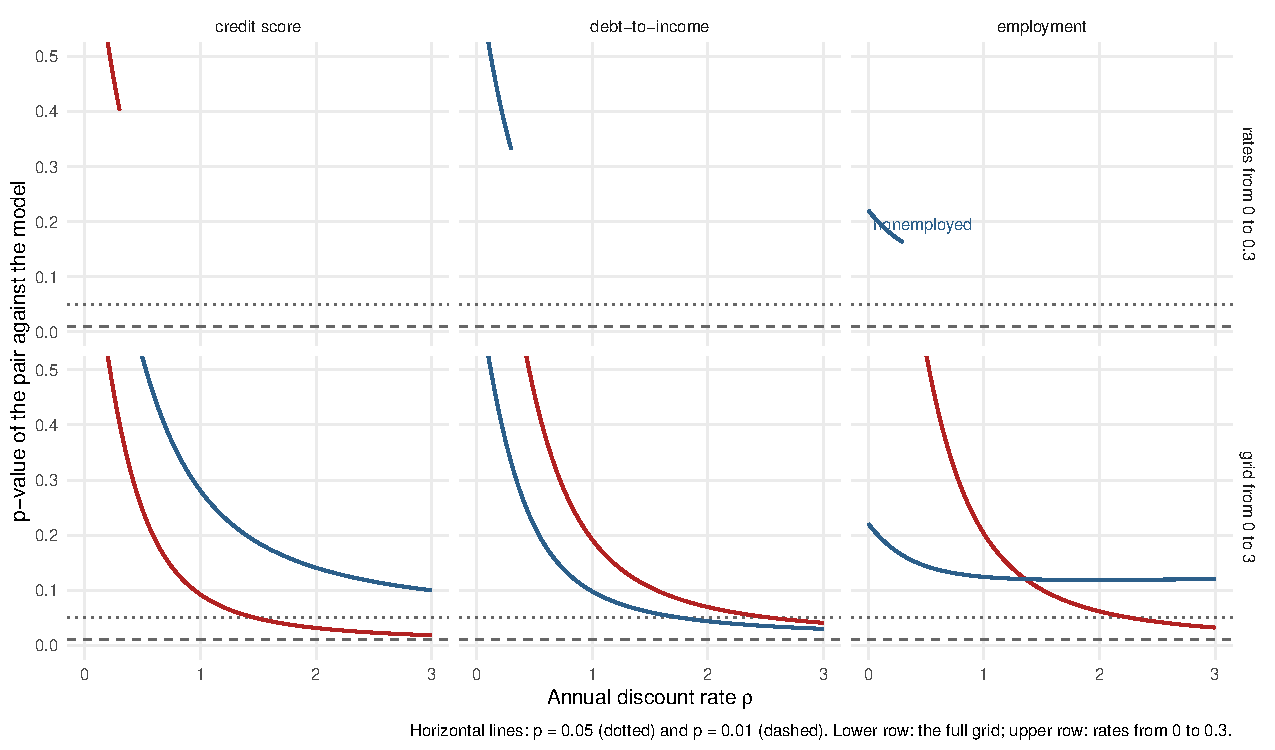
\includegraphics[width=\textwidth]{figures/fig_rho_subgroups.pdf}
\caption{The discount rate by subgroup in the Dobbie--Song experiment. Each curve is the $p$-value of the subgroup's pair of arms against the model's line on the grid of the annual rate from 0 to 3, aggregated over the five-year window at the marginal-utility profile, with survival from the study's exit hazards; the upper row repeats the lower on rates from 0 to 0.3; the dotted and dashed lines are five and one percent.}
\label{fig:rho_subgroups}
% replication: Code/local/experiments_rho_subgroups.R, Code/exhibits/make_rho_subgroups.R
\end{figure}

\begin{table}[H]
\centering
\caption{The discount rate by subgroup in the Dobbie--Song experiment}
\label{tab:rho_subgroups}
\small
\resizebox{\textwidth}{!}{\begin{tabular}{lrrrrrrll}
\toprule
Subgroup & write-down & payment reduction & $\rho$ best fit & $p$ at 0.02 & $p$ at the estimate & $p$ at 0.22 & $\rho$ consistent at 5\% & at 1\% \\
\midrule
All enrollees & $-0.030$ (0.009) & $+0.023$ (0.011) & 0.00 & 0.925 & 0.734 & 0.538 & [0.00, 1.20] & [0.00, 2.84] \\
Debt-to-income above median & $-0.035$ (0.012) & $+0.022$ (0.014) & 0.11 & 0.835 & 0.996 & 0.806 & [0.00, 2.54] & [0.00, 3.00] \\
Debt-to-income below median & $-0.023$ (0.011) & $+0.024$ (0.013) & 0.00 & 0.633 & 0.514 & 0.398 & [0.00, 1.76] & [0.00, 3.00] \\
Credit score above median & $-0.027$ (0.013) & $+0.018$ (0.014) & 0.07 & 0.924 & 0.947 & 0.800 & [0.00, 3.00] & [0.00, 3.00] \\
Credit score below median & $-0.032$ (0.011) & $+0.027$ (0.014) & 0.00 & 0.816 & 0.656 & 0.495 & [0.00, 1.47] & [0.00, 3.00] \\
Employed at baseline & $-0.035$ (0.010) & $+0.019$ (0.012) & 0.20 & 0.647 & 0.829 & 0.954 & [0.00, 2.26] & [0.00, 3.00] \\
Not employed at baseline & $-0.002$ (0.016) & $+0.028$ (0.018) & 0.00 & 0.215 & 0.194 & 0.174 & [0.00, 3.00] & [0.00, 3.00] \\
\bottomrule
\end{tabular}
}
\vspace{0.5em}
\begin{minipage}{0.95\textwidth}
\small \textit{Notes:} Effects on bankruptcy within five years of the maximum-intensity write-down and payment-reduction arms, by subgroup, from \citet{dobbie_targeted_2020}, Table 8 and Appendix Table A9 (standard errors in parentheses). The remaining columns test each pair against the model's line on the grid of the annual rate from 0 to 3 by 0.01, aggregated over the five-year window at the marginal-utility profile, with survival from the study's exit hazards and the two arms treated as independent, their covariance not being reported: the best-fitting rate, the $p$-value at the 2 percent social discount rate, at the paper's estimate and at the laboratory median of 0.22, and the sets of rates not rejected at the five and one percent levels. A set with two components has its second component in the region of high rates where the model predicts no write-down response. The pooled row uses the maximum-arm effects.
\end{minipage}
% replication: Code/local/experiments_rho_subgroups.R, Code/exhibits/make_rho_subgroups.R; results/experiments_rho_subgroups.csv
\end{table}

\subsection{Posterior summaries under a flat prior}

Turned into posterior weights under a flat prior, the estimates of Section \ref{sec:quasi} depend on the prior's support in a way that the $p$-value curve does not (Table \ref{tab:rho_posterior}). On the support $[0, 1]$ the Dobbie--Song posterior has its mode at zero, a mean of $0.36$, a 68 percent highest-density set of $[0, 0.47]$ and a 95 percent set of $[0, 0.88]$. On the support $[0, 3]$ the mode is again zero, but the mean is $0.66$ and a fifth of the posterior mass lies above $\rho = 1$, in the region where the write-down is predicted to do little: the mass is the prior's, not the experiment's, because a flat prior over a wide region of low likelihood accumulates weight that no point in the region earns. Pooling the pair with Ganong--Noel's under one rate changes little on either support, since the second pair's likelihood is nearly flat: the pooled mean is $0.40$ on $[0, 1]$ and $0.72$ on $[0, 3]$, with 68 percent sets of $[0, 0.51]$ and $[0, 0.80]$. The mean of a posterior is not the right summary of this evidence, and the paper does not report one as its rate; the experimental statement of the paper is the Dobbie--Song pair's $p$-value curve, and the check is the set it accepts.

\begin{table}[H]
\centering
\caption{Posterior summaries of the rate under a flat prior, by pair and support}
\label{tab:rho_posterior}
% replication: Code/local/experiments_rho_posterior.R, Code/exhibits/make_rho_posterior_table.R; results/experiments_rho_posterior.csv
\small
\begin{tabular}{llrrll}
\toprule
Pair & Support & Mode & Mean & 68\% set & 95\% set \\
\midrule
Dobbie--Song & $[0, 1]$ & 0.00 & 0.36 & $[0, 0.47]$ & $[0, 0.88]$ \\
Dobbie--Song & $[0, 3]$ & 0.00 & 0.66 & $[0, 0.72]$ & $[0, 2.17]$ \\
Ganong--Noel & $[0, 1]$ & 1.00 & 0.53 & $[0.37, 1]$ & $[0.07, 1]$ \\
Ganong--Noel & $[0, 3]$ & 3.00 & 1.54 & $[1.02, 3]$ & $[0.20, 3]$ \\
Pooled & $[0, 1]$ & 0.16 & 0.40 & $[0, 0.51]$ & $[0, 0.89]$ \\
Pooled & $[0, 3]$ & 0.16 & 0.72 & $[0, 0.80]$ & $[0, 2.24]$ \\
\bottomrule
\end{tabular}

\vspace{0.5em}
\begin{minipage}{0.95\textwidth}
\small \textit{Notes:} Posterior weights $\propto \exp(-\chi^2(\rho)/2)$ on the grid of $\rho$ by $0.01$, under the window aggregation of equation \eqref{eq:window} at the marginal-utility profile, with survival from each study's exit hazards and the arms independent; the pooled row sums the Dobbie--Song (maximum arms) and Ganong--Noel $\chi^2$ statistics. Sets are highest-density sets, the grid points of largest weight that together hold 68 or 95 percent, and are unions of intervals where the posterior has a second region of weight at high rates. The posterior mass above $\rho = 1$ on the $[0, 3]$ support is 0.22 for Dobbie--Song, 0.69 for Ganong--Noel and 0.24 pooled.
\end{minipage}
% replication: Code/local/experiments_rho_posterior.R, Code/exhibits/make_rho_posterior_table.R; results/experiments_rho_posterior.csv
\end{table}

\subsection{Payment paths and $p$-value curves}

\begin{figure}[H]
\centering
\caption{Rule-based experiments as payment-path treatments}
\label{fig:ledger_paths}
% replication: Code/exhibits/make_ledger_figures.R; external/experiments_paths.csv, external/experiments_estimates.csv
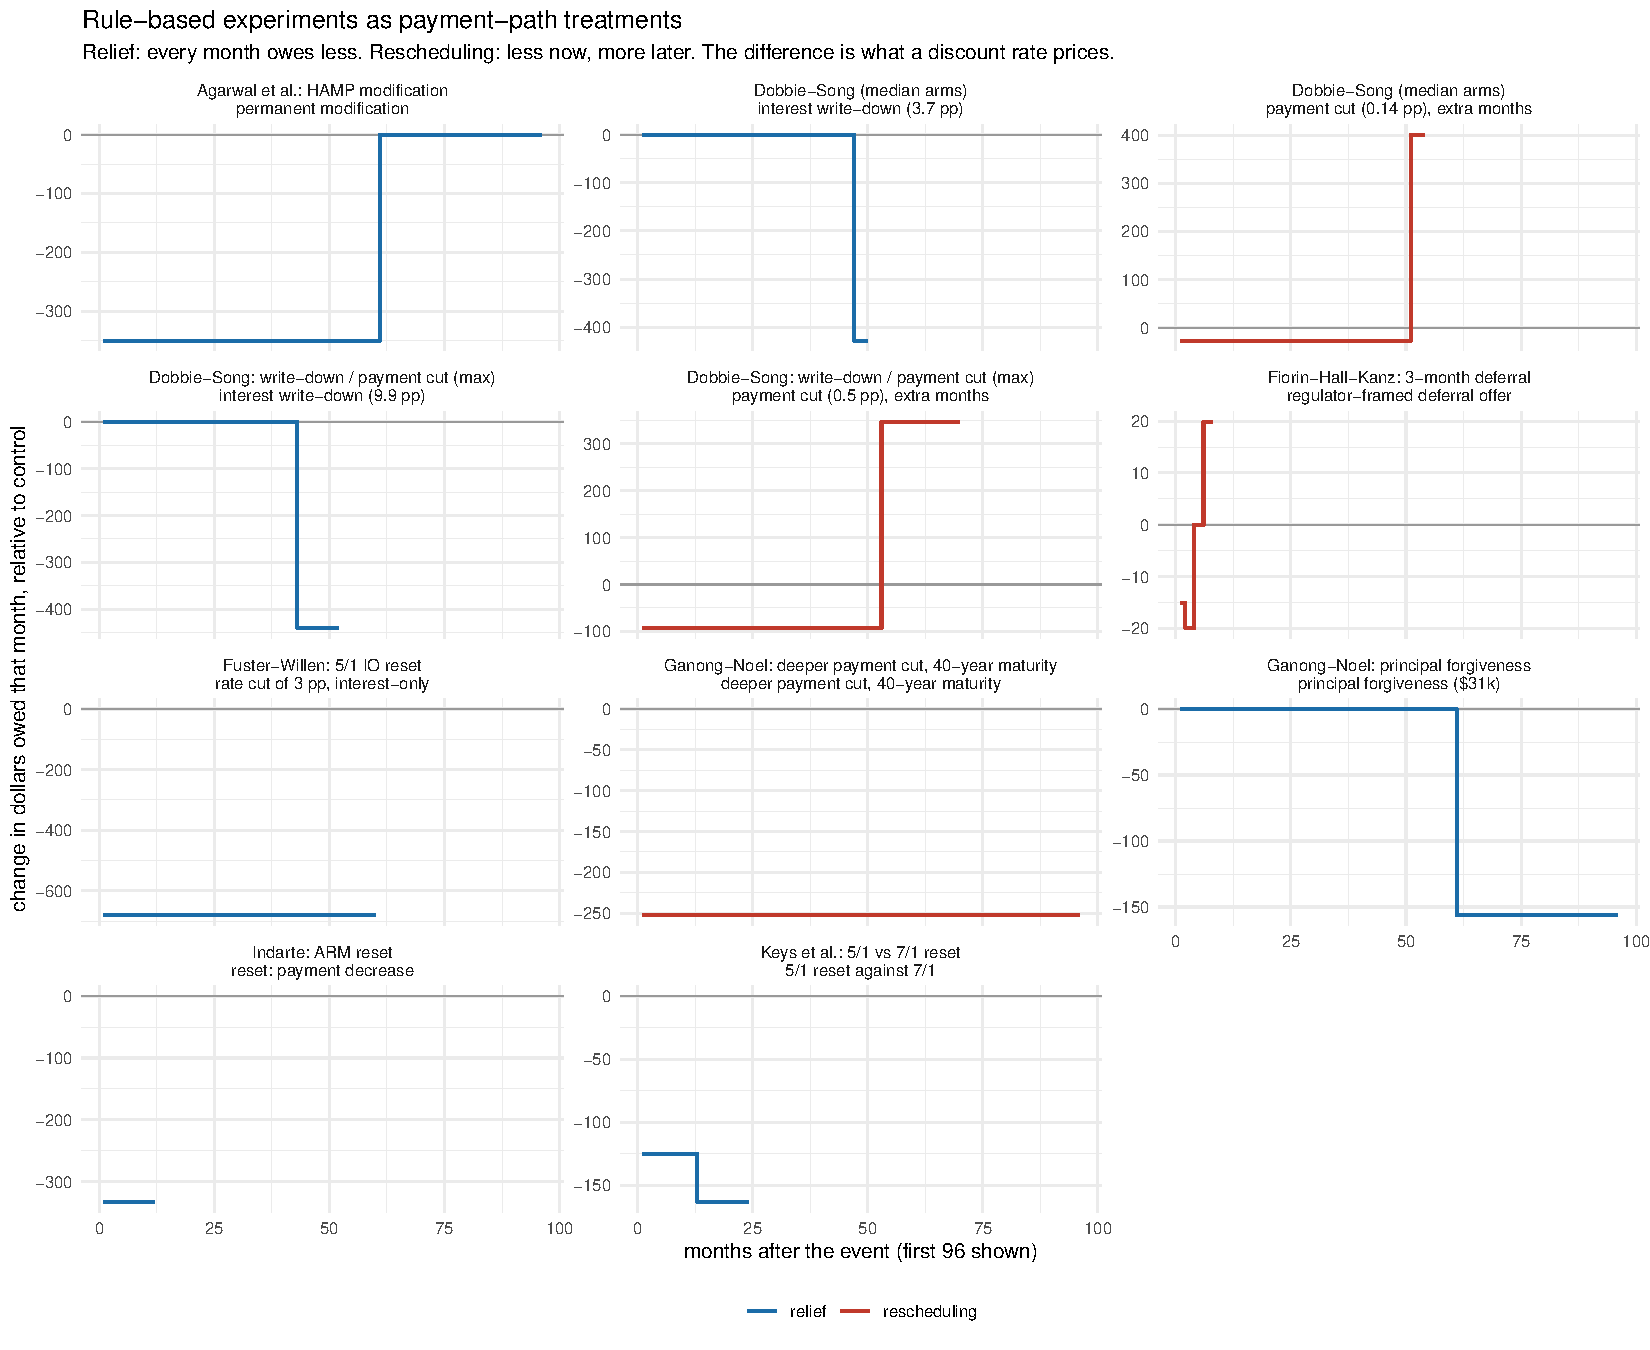
\includegraphics[width=\textwidth]{figures/fig_ledger_paths.pdf}
\begin{minipage}{0.95\textwidth}
\small \textit{Notes:} Each panel is one treatment arm: the change in dollars owed in each month after the event relative to the study's control (first 96 months shown). Blue: relief, every month owes less. Red: rescheduling, less now and more later. The studies shown are those of Table \ref{tab:experiments}. Source: \texttt{external/experiments\_paths.csv}.
\end{minipage}
\end{figure}

\begin{figure}[ht]
\centering
\caption{What each pair of arms says about the discount rate, and the near-horizon response across settings}
\label{fig:ledger_rho}
% replication: Code/exhibits/make_ledger_figures.R, Code/exhibits/make_lambda_figure.R; results/experiments_rho.csv, external/experiments_estimates.csv
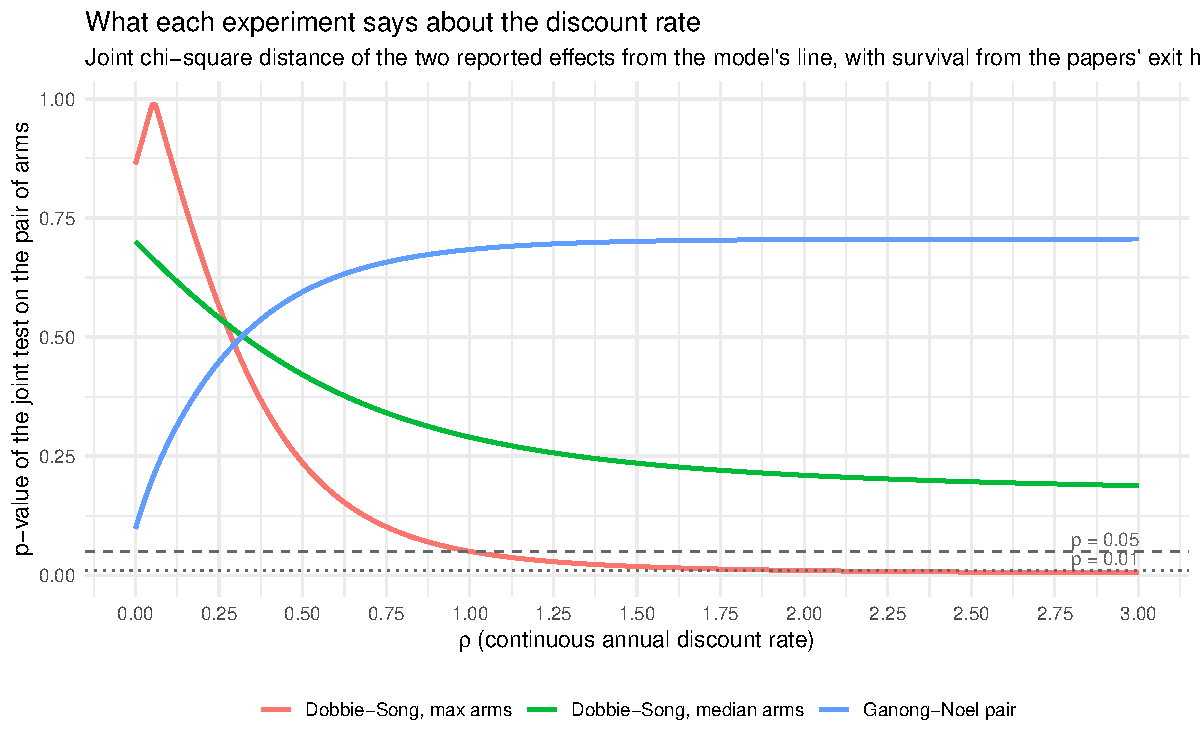
\includegraphics[width=0.8\textwidth]{figures/fig_ledger_rho.pdf}\\[0.5em]
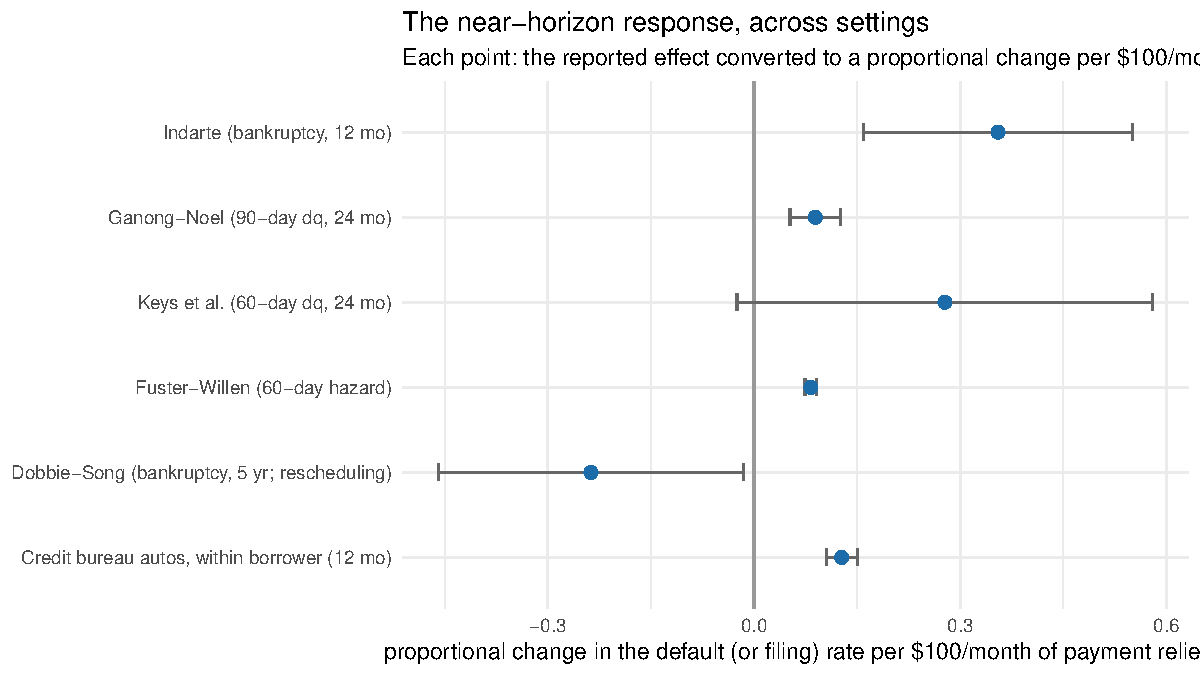
\includegraphics[width=0.8\textwidth]{figures/fig_ledger_near.pdf}\\[0.5em]
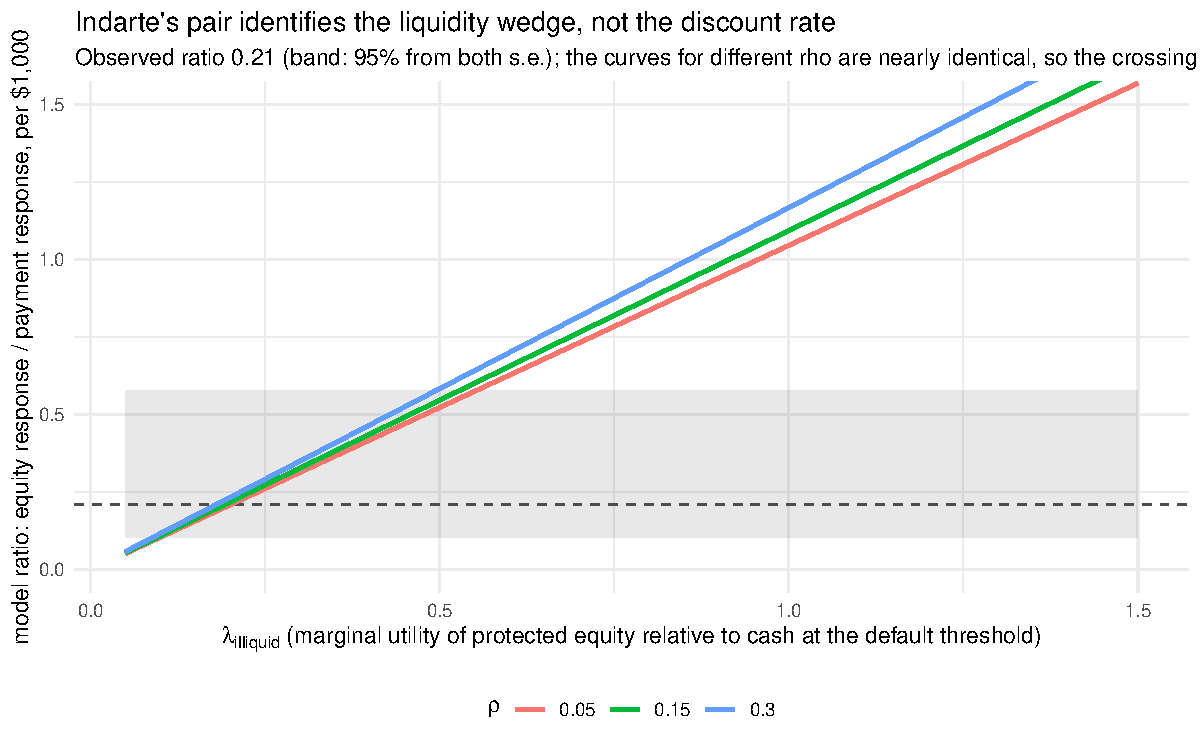
\includegraphics[width=0.8\textwidth]{figures/fig_ledger_lambda.pdf}
\begin{minipage}{0.95\textwidth}
\small \textit{Notes:} Upper panel: the $p$-value of the joint test of a pair of arms against the model, on the grid of $\rho$ from 0 to 3 (Section \ref{sec:mapping}; aggregated over each study's outcome window; survival from each study's exit hazards; the marginal-utility profile; the dashed and dotted lines are five and one percent). Middle panel: each study's reported response converted to a proportional change in the default or filing rate per \$100 a month of payment relief, with the credit-bureau within-borrower payment elasticity at a \$400 payment for comparison. Bottom panel: Indarte's pair, the ratio of the seizable-equity response to the payment response, as the model produces it for values of $\lambda_{\text{illiquid}}$ at three discount rates; the observed ratio crosses at about 0.2 whatever $\rho$ is.
\end{minipage}
\end{figure}

